\documentclass[10pt]{sig-alternate-05-2015}
%\usepackage{pdfpages}
%\usepackage{flushend}
\usepackage{lipsum}
\usepackage{subcaption}
\usepackage{xcolor}
\usepackage{hyperref} 
\usepackage{hypcap}

\begin{document}
\title{Online Communication Traces in Android Memory}

\numberofauthors{8}
\author{
J{\o}rgen Ellingsen, Espen Kjellstadli Lund, Ingrid Johanne Kjesbu Larsen, Jan Petter Berg Nilsen,\\
Emil Volckmar Ry, Anders Sefjord Torbj{\o}rnsen, Magnus Omland Torgersen, Torstein Ryland Grotle
\\\{jorgeell, espenklu, ingridjl, jpnilsen, emivr, andetorb, magnuoto, torsterg\}@stud.ntnu.no
}

\maketitle
\begin{abstract}
All data are at some point present in memory, but this paper examines what traces of communication survives in memory after the application is closed down. To examine this an Android phone was filled with some of the most used communication applications on the market, and engaged in communications through these. It was then rooted without a reboot and connected to a computer for memory extraction. A market top-selling cleaning tool was also downloaded and ran between data creation and extraction to do as much as a every-day user could practically do to remove communication traces from memory. The experiment had some limitations since we had to root the phone, and we had all the credentials for the phone. Additionally the phone was not in daily use, and only used during the experiment. The extraction showed traces from all of the used applications except Jodel. From Snapchat we found partial images and thumbnail of sent and received images, from Facebook Messenger and Whatsapp we found all communications, and after a map address search we found both the address and the current location of the phone. This showed that a lot of information is accessible in the memory after the application is closed, and this information could persist for a long time depending on the usage and memory requirements of applications run between the generation and the extraction. 
\end{abstract}

\keywords{Android; Memory; Forensics; Practical approach}

\section{Introduction}
Today the battery life of smartphones has reached the point that even with all the usage we do on our phones today, it will in most cases last the entire day. As a result of this, a smartphone can stay on for weeks, or even months at a time and old information can still be present in the memory. As most of our communication today are done with mobile applications like Facebook, GMail and Snapchat this project tries to analyse what information is stored in memory, and how long it is recoverable for the different applications. \\ \\
For data to be used by the processor in a smart phone it has to be present in memory while being presented or used. This project aims to examine what happens when the application is closed, and the data is no longer in use. For the traces to be gone the memory must not only be freed up for other applications to use, but overwritten by new data. If not, the data will survive until the device is rebooted or new applications allocate and overwrite the now free space. Additionally, some applications claim to have features like anonymity and auto-delete functionality, and applications like this should take extra care to make sure there are no fragments of the communication left in memory after the application is closed.
\\ \\
\begin{tabular}{ |p{3cm}|p{4.5cm}|  }
 \hline
 \multicolumn{2}{|c|}{\textbf{Definitions}} \\
 \hline
 Root, Rooting&Gaining privileges beyond what is intended by the manufacturer, effectively super-user or root (UNIX) \\
 \hline
  Memory Dump& Bit-by-bit copy of the device's random access memory.\\
 \hline
 Carving& Searching a memory dump for  files based on content, rather than on metadata.\\
 \hline
 Regular Expression & Powerful pattern searching technique.\\
 \hline
 JSON & JavaScript Object Notation is form of organizing structured data in a string form.\\
 \hline
 SSID & Service Set Identifier is a unique identifier attached to the header of packets sent over a wireless local-area network .\\
 \hline
\end{tabular}

\clearpage

\section{Background}
Many of todays smart phones are running Android as their operating system, and  data claims it dominates the market with an 87.6\% share in the second quarter of 2016\cite{idc}. Making it essenstial for future mobile forensic work, for gathering information in an investigation.

When an investigation occurs, there are several approaches to data acquisistion: (1) Manual acquisition, (2) Logical acquisition, (3) Physical acquisition, (4) Brute force acquisition. The field of interest for this paper is physical acquisition of the primary storage; it focuses primarly on creating a bit-by-bit copy of the random access memory (RAM). Due to RAM being volatile, it is often the target of stealthy illegal activites to avoid leaving data. If data was stored in the flash drive, it would still be resident until OS tries to overwrite the same physical area and garbage collector is initiated. The point being that data residing on a secondary storage device, will be living longer and probably be logged more extensively.

The Android OS is in short words a Linux-based OS, where most OS tasks are performed by open source C libraries, and Java is used for the development of Android applications. These applications are compiled to bytecode for the Java virtual machine (JVM), which is then translated for a second virtual machine which executes them. Depending on which version of Android a smart phone is running, different virtual machines are used for execution.
For Android versions 4.4 and prior, Dalvik was used. It was replaced by ART in 4.5, and is still the de-facto standard.

Why does this matter? The virtual machines that are used are suppose to run Java applications, and have therefore gained several features of the Java programming language. One of these features are the memory management module, which has a built-in garbage collector(GC). It lets the user create objects without worrying about memory allocation and deallocation. Reducing the need for boilerplate code, and problems with memory leaks and such, which often are languages like C and C++ are subject to. 

The GC have the job of cleaning RAM, therefore removing potential information to be gathered. It is therefore of severe importance, that data residing in memory gets gathered before the device eventually power offs, or the garbage collector initializes.

Both ART and Dalvik use by default a method called "concurrent mark and sweep" for their GC\cite{ARTGC,DALVIKGC}. It works by traversing the heap for objects that are "reachable" or used by applications, those who are not will be regarded as free space again. Making space for potential new data to be stored within it. A figure of the process, can be seen at figure \ref{fig:mas}. Generally the heap is a region of the memory that is regarded as free memory for any process to use, however in Java it is used to store all objects created. Therefore the GC may potentially remove one of the better sources for information, the objects. The good news are that once data is freed, no overwriting is enforced; in other words, data is not overwritten until another object takes its place\cite{DALVIKGC}; in addition to each application running its own garbage collector and private heap, making the RAM data resident for possibly long periods of time\cite{AndroidMemManagement}.

\begin{figure}[h]
  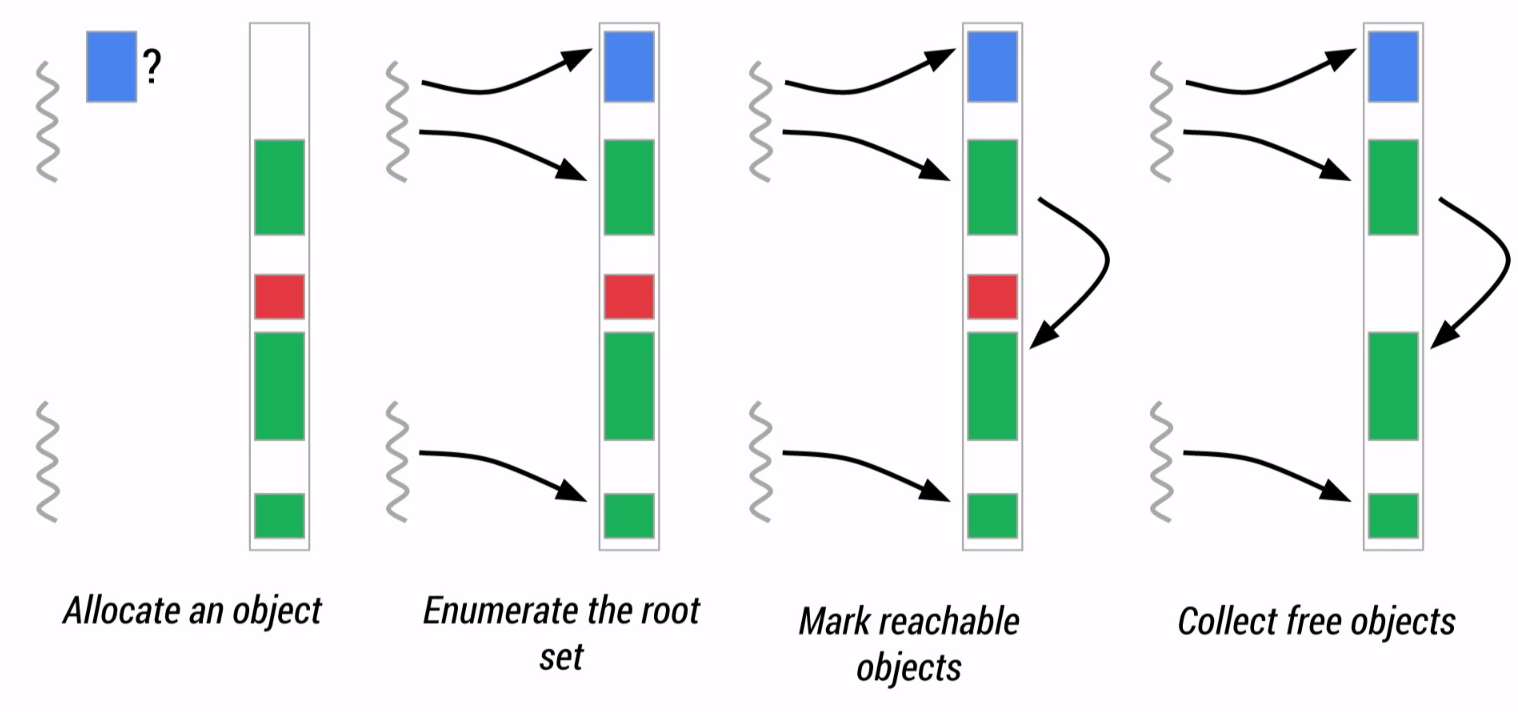
\includegraphics[width=0.5 \textwidth]{gc}
  \caption{Mark and Sweep\cite{ARTGC}}
  \label{fig:mas}
\end{figure}

Because all objects created in the heap, there may be a potential trace of information of an application. Through the use of several popular online communication applications, the amount of data that can be collected through a memory dump will be explored; despite knowing that the GC might start, or extra security measures might prevent us to do so.

\section{Practical Application}
%\lipsum[1-2]
We wanted to find remaining traces in memory from communication data and application metadata. For this we used the phone Sony Xperia M2 with Android 5.1.1.

\subsection{Laboratory Environment}
The phone was factory reset to ensure a reproducible result. At this point the phone was rooted %TODO: Explain term
using the KingRoot application version 4.9.5. This process did not require restart of the phone, potentially leaving traces of memory from before rooting and making it ideal for memory forensics provided the phone can be unlocked regardless of root status. After testing the root, the phone was restarted to ensure a consistent state. As part of this process ADB USB debugging was enabled. A memory cleaning app was installed which promised \textbf{INGRID: to wipe the memory, xy.z}

We used this tool because we wanted to check if data could survive a cleaning tool. Since we couldn't test over longer periods of time, and since the phone had very low memory\textbf{TTL memory, JP}, we used a cleaningtool to provide a more realistic environment with lot of use. 

Several applications was installed for testing. The applications installed were:
\begin{description}
\item[Facebook]
\item[Facebook Messenger]
\item[Snapchat]
\item[WhatsApp]
\item[Jodle]
\item[Google Apps] \hfill\\Preinstalled on the phone, including GMail, Maps and Chrome
\end{description}
Since this was performed after rooting of the phone, testing of remains in memory when rooting was impossible.

Github was accessed using the Chrome browser.
%Some services were accessed using the Chrome browser:
%\begin{description}
%\item[GitHub]
%\end{description}
\subsubsection*{Approach for each application}
\subsection{Process} %TODO: Bedre navn
This section outlines the steps used for preparing the services and applications for memory forensics.

\subsubsection{Creation of credentials}
We created user accounts corresponding to individual applications. A full list is below.\\
\begin{table}
\begin{tabular}{l|l|l}
Service & User Name & Password \\ 
\hline 
Facebook & mis2016forensics@gmail.com & hackmyphone01 \\ 
Snapchat & canuhackmyphone & hackmyphone07 \\ 
WhatsApp & [Phone number] & - \\ 
Google & mis2016forensics@gmail.com & hackmyphone \\ 
Github & canuHackmyphone & hackmyphone06 \\ 
\end{tabular} 
\caption{Credentials used}
\label{tbl:credentials}
\end{table}

The credentials for whatsapp has been removed from the list, however a normal phone number was used, together with a password.

After creation of the accounts in the applications, the account was used to authenticate with the applications.
% Create User accounts
% Log in to user accounts

\subsubsection{Creating searchable data}
In each of the applications, a normal session was fabricated with easily searchable data.
The types of data used for each application is specified below:
\begin{description}
\item[Facebook] \hfill\\
Information about user and friends.
\item[Facebook messenger]\hfill\\
Unique random strings and images from camera taken in application.
\item[Snapchat]\hfill\\
Images from camera taken in application.
\item[WhatsApp]\hfill\\
Unique strings and images from camera taken in application.
\item[GMail]\hfill\\
Unique random strings and images from camera taken in application.
\item[Google Chrome]\hfill\\
Credentials to GitHub. Web history.
\item[Google Maps]\hfill\\
GPS data, locations and route between locations.
\end{description}
In addition to the data listed, credentials as stored by the application is present.

\begin{figure}[h]
\centering
 \begin{subfigure}[b]{0.15\textwidth}
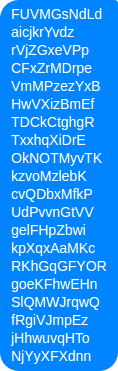
\includegraphics[width=\textwidth]{figures/messenger_string}
\caption{Messenger}
\end{subfigure}
 \begin{subfigure}[b]{0.2\textwidth}
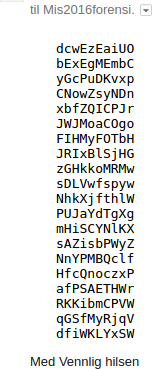
\includegraphics[width=\textwidth]{figures/random_string_in_gmail}
\caption{GMail}
\end{subfigure}
\caption{Example of string used}
\end{figure}
% Send messages using the apps
% Receive messages

% Strings used
% Use of graphic images



\subsubsection{Extracting memory}
To extract the memory AMExtract was chosen. %TODO: REF
 It did not have a profile for the phone, so a profile for extraction method, size of %TODO: name of buffer
 and other properties was created and tested.
 
 The tool was then compiled using the ndk-build tool. As part of the linux kernel headers has been modified, one of the types had to be redefined using an older header file.

\subsubsection{Searching memory}
The extracted memory was searched using the credentials from table\ref{tbl:credentials} and strings which was previously entered. For this purpose the 'strings' tool was used to extract continuous regions of ASCII text and 'grep' was used to search in this text. This has the disadvantage of only finding continuous buffers using simple storage mechanisms, but is quick to execute.

\subsubsection{Carving memory}
To find other types of resources a simple file carving was attempted using 'scalpel' with matches for the following file types:
\begin{itemize}
	\item PNG
	\item JPG
	\item TIFF
\end{itemize}

\subsection{What were we looking for}
\lipsum[7]

\section{Results}
\begin{table}[!ht]
\centering
\begin{tabular}{|m{1.8cm}|m{2.5cm}|m{3cm}|}
\hline
Search phrase & Description & Findings \\
\hline
http:// & Attempting to find web related data  & Traces of communication and general use. Most specific information was facebook communication requests with names. \\
\hline
'60\textbackslash.[0-9]*,10\textbackslash.[0-9] *' &  RegEx for GPS coordinates in the area & Our specific location, as well as the location of our search target \\
\hline
password & A generic search for string "password" & Found passwords saved in browser, specified in table \ref{spesificS_table}. \\
\hline
'\{\}' & Generic JSON search & Complete Facebook information of correspondents: messages, user names and IDs, full profile pictures\\
\hline  
wifi & Generic search for wifi connections & Connection details including SSIDs \\  
\hline
fbpushnotif & String used in Facebook push notifications & List of notifications sent to the phone.\\
\hline
facebook: & String used in Facebook activity & Messages, their participants and other activity. Lots of JSON data.\\
\hline
\end{tabular}
\caption{Table of generic searches and findings}
\label{genericS_table}
\end{table}

In this section we explore our findings, what we expect to find, what we did find and other information we found. 

\subsection{Results from generic search terms}
When searching for generic information and structures, some structured information was found. This included JSON when searching for '\{' and http requests when searching for 'http://'.\\\\
A search for coordinates matching the shown regular expression was performed, which corresponds to the area the phone was located. Matches for a location in Google Maps was returned with the street address. This was from a search performed in the Google Maps application during the preparation. Searching for part of the address string revealed the address at different stages of completion.\\\\
The findings from generic search terms can be found in table \ref{genericS_table}.

\subsection{Results from specific key phrases}
The passwords and usernames from table \ref{tbl:credentials} was used to detect the presence of credentials. Results are in the following table \ref{spesificS_table}. Some applications are not included due to not having any credentials, such as Jodel and Google Maps.\\
\begin{table}[h]
\centering
\begin{tabular}{|m{2.5cm}|m{2.5cm}|m{2.5cm}|}
\hline
App & Description & Findings \\
\hline
Facebook and Messenger & Username and password & Found username.  \\
\hline
Snapchat & Username and password & Found nothing. \\
\hline
WhatsApp & Phone number & Found phone number. \\
\hline 
Google (Gmail) & Email and password & Found email.\\
\hline
Google Chrome (GitHub password saved in browser) & Username and password. & Found username and password \\
\hline
Wifi & Wifi name and password & Found name. Found password but without context to relate them.\\  
\hline
SSID & Searched for wifi names the device had been around & Found SSID of discovered networks, but not much context.  \\  
\hline
\end{tabular}
\caption{Table of searches and findings (credentials)}
\label{spesificS_table}
\end{table}
\\For finding information related to Facebook, a case-insensitive search for the string Facebook was performed. This revealed information about friends of the logged in user, metadata of other users profile pictures was found from the Facebook application along with chat messages from Facebook Messenger. Information regarding whether the contact was muted, timestamp of last delivery and timestamp of last confirmed received message by the other participant. Searching for the name of the participants could identify the chat messages, since all the messages had metadata containing name of the other party.\\
For GMail and e-mail messages, the content and metadata was often found in the memory dump. As such the messages could be found by searching for the e-mail address.
%For the applications which has been provided with a unique string

\subsection{Carved images}
When carving several images were recovered. Most of these where part of stock Android OS or part of an applications assets, however when matching JPEG images, several of the pictures taken by the camera was discovered. These had no metadata. A overview of what was returned from each application can be found below:
\begin{description}
\item[Camera]\hfill\\
The full scale image was only available for a short duration after use before being stored on the device, however a small scale preview from the select image screen or camera was still in memory.
\item[WhatsApp]\hfill\\
No images could be recovered, however a reference to a file name of the image could be found in the chat conversation from memory suggesting it is stored on the device.
\item[Snapchat]\hfill\\
The full scale image was only available for a short duration after use. After some time part of the memory region containing the image was overwritten by a sequence of zeroes before finally being removed entirely, however a small scale preview from the select image screen or camera was still in memory.
\end{description}

\section{Discussion}
%Rooted without rebooting
%Unallocated data, and partially overwritten
%Limitations
%Full access to the phone
%Phone memory size
%Timeframe
%1GB memory, 800MB dump
%Writeblock
%Kingroot - what does it do?
%Forensic process
To perform the memory dump, a preliminary research was initiated to discover tools compatible with the smartphone's software; where the criteria were: easy to perform, and minimal alteration of memory. Two different tools were encountered, namely Odin and KingRoot. Both ensure that the phone is rooted, which enable memory dump functionality.\\\\
It was unfortunately discovered that Odin was not up to the task, it required: an application to be installed on a computer, a USB connection, and a reboot of the phone was required. Because it requires a reboot, memory content is lost. On the other hand, KingRoot granted root access without rebooting and is therefore preferred. Nevertheless, it is not recommended to use KingRoot in a forensic case, due to the fact that the application alters the memory unpredictably. The main cause being that the application is proprietary technology, thus problematic to examine how it interacts with the system. Consequently, if this research was to be done in a more forensics setting, different methods or tools would have been reconsidered.
\subsection{Limitations}
As already mentioned, it is difficult to determine how memory is altered in the process of extracting data; due to the nature of how RAM is used in operating systems and lack of documentation. Moreover, data is dynamic and may get erased at any time. In comparison, it is far easier to block writing to hard drives with write blockers. For this reason, a limitation with the process is how integrity of data is not preserved.\\\\
Other limitations that influence our results are: a limited memory pool to extract data from, lack of SIM card for additional information, limited time to perform the study, and running all applications of interest at once.

\subsubsection{Timeframe}
Due to the limited time frame, our testing procedure has been condensed to focus on if data would survive a cleaning tool. At first, the aim was to get an idea of how long data might be resident in RAM until overwritten. As a consequence, the scope of the research has been reduced. Despite this, the results did demonstrate that Snapchat pictures only were available for a short duration after use. It does however, create room for other data to be extracted.
\subsubsection{SIM}
The smartphone in use, did not have a SIM card. As a consequence, AMExtractor was unable to extract data about contacts, phone calls, text messages, or information related to cell towers it might have been connected to. Most data had been crafted beforehand, for the sole purpose of being easily searched for.
\subsubsection{Memory}
Despite the smartphone possessing 1GB memory, only 800MB was extracted. A theory of why this is the case, is that there is no direct mapping between the virtual and physical memory. As a result, not all information was retrieved. With a modern phone, more traces would have been acquired. Generally, because they tend to have more RAM than their ancestors. For instance, the latest Google Nexus 6P has 3GB RAM, which is three times more than the one tested\cite{huawei}.
\subsubsection{Unallocated, and partially overwritten data}
Preparation for memory collection, was done by performing various actions within each application of interest. This was done sequentially, which could have resulted in data being overwritten in the RAM. The reason being that the GC freed some of the memory fore reallocation, and as more applications were launched the memory was reallocated for them. As a result, some images that were extracted were partly overwritten and nearly unidentifiable.\\\\
It is likely that the GC probably would have done less damage to data, if more RAM was available. Simply because, the GC is primarily triggered by size limits or collision detection.
\subsubsection{Forensic Process}
The forensic phase did not follow best practice. A JTAG approach, may have been a better approach to keep data integrity but was impractical for this study. Furthermore, no specialized tools were used to perform the analysis of extracted data; the command-line utility grep was used. It is therefore likely that a more suited tool, may have given us the opportunity to find more data of relevance. Also, it cannot be confirmed that the phone has been tampered with during the process. It is unlikely, but not provable.\\

\section{Conclusion}
Data privacy is more important than ever, as adoption of smartphones keep increasing. This project has shown that with a few steps the amount of private information can be retrieved out of the memory on a mobile phone. First of all to gain root access over the phone was tested with two different programs where one of them did not need the phone to be turned off. That is advantageous in real forensic cases due to the fact that all the memory in the RAM is still intact. With the help of a tool called AMExtract and the linux kernel, we were able to dump the files from the RAM onto our computer. During the forensics process two types of searches was used in order to examine the information. A generic search with the keyword HTTP lead to us finding the GPS coordinates of the previous google maps search on the phone. The second type of search was a more specific search with the keyword Facebook. This gave us conversations done on Facebook with the timestamps of the various messages. With the previous findings we tried a cleaning tool while closing the applications used. The result of this was little to nothing and had no impact of the information that was dumped. One of the more interesting result of our forensic process was the dumped information by the application Snapchat. Shortly after using Snapchat and dump the memory on to our computer, we found a full scale image that was taken in Snapchat. After a while the memory containing the image was overwritten, nonetheless a small scale preview of the image was still in memory. While all of our findings was fascinating, the GPS coordinates and the Facebook conversations was by far the most interesting. That kind of information can be used in real forensic cases.

\bibliographystyle{vancouver}

\bibliography{b}  

\end{document}
